\section{Huvudmodul}
Huvudmodulen kan ses som systemets "hjärna". Här sker alla beräkningar för att roboten ska kunna utföra sina uppgifter. Dessa uppgifter ska huvudmodulen hantera antingen via kommandon från en PC eller skötas helt autonomt. Detta är en kritisk modul då den kommer att utföra mycket uppgifter. Den behöver inte mycket hårdvara men den kommer vara mjukvarutung.
\subsection{Hårdvara}
Modulen ska förslagsvis bestå av en enkortsdator av modell Beagleboard. Den har en ARM Cortex-A8 processor som har en klockfrekvens på 1GHz. Denna behöver ett operativsystem för att kunna användas. Den enda hårdvaran som behövs för att kunna använda BB är ett minneskort för operativsystem och en bluetooth-dongel för kommunikationen med PC:n. Även två USB-UART konverterare behövs för kommunikationen med de övriga modulerna.
\subsection{Mjukvara}
% Graphic for TeX using PGF
% Title: /home/martin/Downloads/trådar.dia
% Creator: Dia v0.97.2
% CreationDate: Mon Oct  6 14:56:04 2014
% For: martin
% \usepackage{tikz}
% The following commands are not supported in PSTricks at present
% We define them conditionally, so when they are implemented,
% this pgf file will use them.
\ifx\du\undefined
  \newlength{\du}
\fi
\setlength{\du}{15\unitlength}
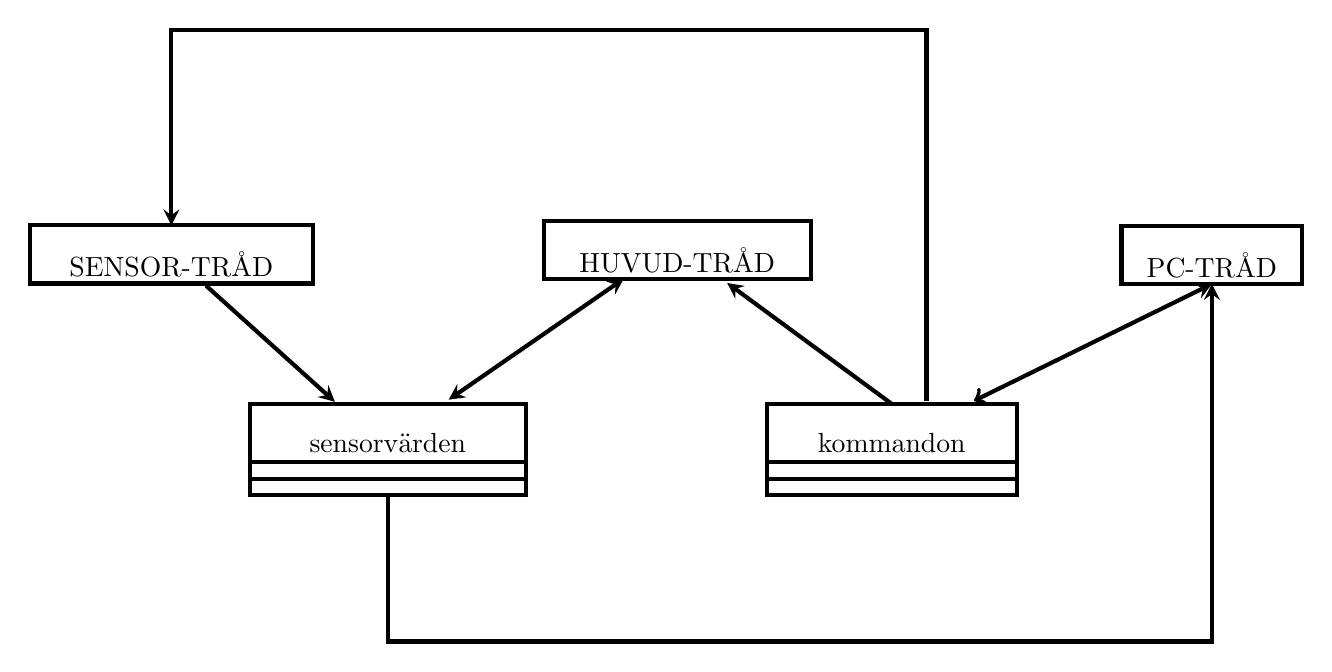
\begin{tikzpicture}
\pgftransformxscale{1.000000}
\pgftransformyscale{-1.000000}
\definecolor{dialinecolor}{rgb}{0.000000, 0.000000, 0.000000}
\pgfsetstrokecolor{dialinecolor}
\definecolor{dialinecolor}{rgb}{1.000000, 1.000000, 1.000000}
\pgfsetfillcolor{dialinecolor}
\pgfsetlinewidth{0.100000\du}
\pgfsetdash{}{0pt}
\definecolor{dialinecolor}{rgb}{1.000000, 1.000000, 1.000000}
\pgfsetfillcolor{dialinecolor}
\fill (83.362742\du,-37.782161\du)--(83.362742\du,-36.382161\du)--(89.792742\du,-36.382161\du)--(89.792742\du,-37.782161\du)--cycle;
\definecolor{dialinecolor}{rgb}{0.000000, 0.000000, 0.000000}
\pgfsetstrokecolor{dialinecolor}
\draw (83.362742\du,-37.782161\du)--(83.362742\du,-36.382161\du)--(89.792742\du,-36.382161\du)--(89.792742\du,-37.782161\du)--cycle;
% setfont left to latex
\definecolor{dialinecolor}{rgb}{0.000000, 0.000000, 0.000000}
\pgfsetstrokecolor{dialinecolor}
\node at (86.577742\du,-36.832161\du){HUVUD-TRÅD};
\pgfsetlinewidth{0.100000\du}
\pgfsetdash{}{0pt}
\definecolor{dialinecolor}{rgb}{1.000000, 1.000000, 1.000000}
\pgfsetfillcolor{dialinecolor}
\fill (70.982742\du,-37.669161\du)--(70.982742\du,-36.269161\du)--(77.805242\du,-36.269161\du)--(77.805242\du,-37.669161\du)--cycle;
\definecolor{dialinecolor}{rgb}{0.000000, 0.000000, 0.000000}
\pgfsetstrokecolor{dialinecolor}
\draw (70.982742\du,-37.669161\du)--(70.982742\du,-36.269161\du)--(77.805242\du,-36.269161\du)--(77.805242\du,-37.669161\du)--cycle;
% setfont left to latex
\definecolor{dialinecolor}{rgb}{0.000000, 0.000000, 0.000000}
\pgfsetstrokecolor{dialinecolor}
\node at (74.393992\du,-36.719161\du){SENSOR-TRÅD};
\pgfsetlinewidth{0.100000\du}
\pgfsetdash{}{0pt}
\definecolor{dialinecolor}{rgb}{1.000000, 1.000000, 1.000000}
\pgfsetfillcolor{dialinecolor}
\fill (76.282742\du,-33.369161\du)--(76.282742\du,-31.969161\du)--(82.932742\du,-31.969161\du)--(82.932742\du,-33.369161\du)--cycle;
\definecolor{dialinecolor}{rgb}{0.000000, 0.000000, 0.000000}
\pgfsetstrokecolor{dialinecolor}
\draw (76.282742\du,-33.369161\du)--(76.282742\du,-31.969161\du)--(82.932742\du,-31.969161\du)--(82.932742\du,-33.369161\du)--cycle;
% setfont left to latex
\definecolor{dialinecolor}{rgb}{0.000000, 0.000000, 0.000000}
\pgfsetstrokecolor{dialinecolor}
\node at (79.607742\du,-32.419161\du){sensorvärden};
\definecolor{dialinecolor}{rgb}{1.000000, 1.000000, 1.000000}
\pgfsetfillcolor{dialinecolor}
\fill (76.282742\du,-31.969161\du)--(76.282742\du,-31.569161\du)--(82.932742\du,-31.569161\du)--(82.932742\du,-31.969161\du)--cycle;
\definecolor{dialinecolor}{rgb}{0.000000, 0.000000, 0.000000}
\pgfsetstrokecolor{dialinecolor}
\draw (76.282742\du,-31.969161\du)--(76.282742\du,-31.569161\du)--(82.932742\du,-31.569161\du)--(82.932742\du,-31.969161\du)--cycle;
\definecolor{dialinecolor}{rgb}{1.000000, 1.000000, 1.000000}
\pgfsetfillcolor{dialinecolor}
\fill (76.282742\du,-31.569161\du)--(76.282742\du,-31.169161\du)--(82.932742\du,-31.169161\du)--(82.932742\du,-31.569161\du)--cycle;
\definecolor{dialinecolor}{rgb}{0.000000, 0.000000, 0.000000}
\pgfsetstrokecolor{dialinecolor}
\draw (76.282742\du,-31.569161\du)--(76.282742\du,-31.169161\du)--(82.932742\du,-31.169161\du)--(82.932742\du,-31.569161\du)--cycle;
\pgfsetlinewidth{0.100000\du}
\pgfsetdash{}{0pt}
\definecolor{dialinecolor}{rgb}{1.000000, 1.000000, 1.000000}
\pgfsetfillcolor{dialinecolor}
\fill (88.732742\du,-33.369161\du)--(88.732742\du,-31.969161\du)--(94.760242\du,-31.969161\du)--(94.760242\du,-33.369161\du)--cycle;
\definecolor{dialinecolor}{rgb}{0.000000, 0.000000, 0.000000}
\pgfsetstrokecolor{dialinecolor}
\draw (88.732742\du,-33.369161\du)--(88.732742\du,-31.969161\du)--(94.760242\du,-31.969161\du)--(94.760242\du,-33.369161\du)--cycle;
% setfont left to latex
\definecolor{dialinecolor}{rgb}{0.000000, 0.000000, 0.000000}
\pgfsetstrokecolor{dialinecolor}
\node at (91.746492\du,-32.419161\du){kommandon};
\definecolor{dialinecolor}{rgb}{1.000000, 1.000000, 1.000000}
\pgfsetfillcolor{dialinecolor}
\fill (88.732742\du,-31.969161\du)--(88.732742\du,-31.569161\du)--(94.760242\du,-31.569161\du)--(94.760242\du,-31.969161\du)--cycle;
\definecolor{dialinecolor}{rgb}{0.000000, 0.000000, 0.000000}
\pgfsetstrokecolor{dialinecolor}
\draw (88.732742\du,-31.969161\du)--(88.732742\du,-31.569161\du)--(94.760242\du,-31.569161\du)--(94.760242\du,-31.969161\du)--cycle;
\definecolor{dialinecolor}{rgb}{1.000000, 1.000000, 1.000000}
\pgfsetfillcolor{dialinecolor}
\fill (88.732742\du,-31.569161\du)--(88.732742\du,-31.169161\du)--(94.760242\du,-31.169161\du)--(94.760242\du,-31.569161\du)--cycle;
\definecolor{dialinecolor}{rgb}{0.000000, 0.000000, 0.000000}
\pgfsetstrokecolor{dialinecolor}
\draw (88.732742\du,-31.569161\du)--(88.732742\du,-31.169161\du)--(94.760242\du,-31.169161\du)--(94.760242\du,-31.569161\du)--cycle;
\pgfsetlinewidth{0.100000\du}
\pgfsetdash{}{0pt}
\definecolor{dialinecolor}{rgb}{1.000000, 1.000000, 1.000000}
\pgfsetfillcolor{dialinecolor}
\fill (97.282742\du,-37.657161\du)--(97.282742\du,-36.257161\du)--(101.635242\du,-36.257161\du)--(101.635242\du,-37.657161\du)--cycle;
\definecolor{dialinecolor}{rgb}{0.000000, 0.000000, 0.000000}
\pgfsetstrokecolor{dialinecolor}
\draw (97.282742\du,-37.657161\du)--(97.282742\du,-36.257161\du)--(101.635242\du,-36.257161\du)--(101.635242\du,-37.657161\du)--cycle;
% setfont left to latex
\definecolor{dialinecolor}{rgb}{0.000000, 0.000000, 0.000000}
\pgfsetstrokecolor{dialinecolor}
\node at (99.458992\du,-36.707161\du){PC-TRÅD};
\pgfsetlinewidth{0.100000\du}
\pgfsetdash{}{0pt}
\pgfsetdash{}{0pt}
\pgfsetbuttcap
{
\definecolor{dialinecolor}{rgb}{0.000000, 0.000000, 0.000000}
\pgfsetfillcolor{dialinecolor}
% was here!!!
\pgfsetarrowsstart{stealth}
\pgfsetarrowsend{stealth}
\definecolor{dialinecolor}{rgb}{0.000000, 0.000000, 0.000000}
\pgfsetstrokecolor{dialinecolor}
\draw (81.072842\du,-33.469161\du)--(85.291242\du,-36.382161\du);
}
\pgfsetlinewidth{0.100000\du}
\pgfsetdash{}{0pt}
\pgfsetdash{}{0pt}
\pgfsetbuttcap
{
\definecolor{dialinecolor}{rgb}{0.000000, 0.000000, 0.000000}
\pgfsetfillcolor{dialinecolor}
% was here!!!
\pgfsetarrowsend{stealth}
\definecolor{dialinecolor}{rgb}{0.000000, 0.000000, 0.000000}
\pgfsetstrokecolor{dialinecolor}
\draw (75.225188\du,-36.219869\du)--(78.331671\du,-33.419491\du);
}
\pgfsetlinewidth{0.100000\du}
\pgfsetdash{}{0pt}
\pgfsetdash{}{0pt}
\pgfsetmiterjoin
\pgfsetbuttcap
{
\definecolor{dialinecolor}{rgb}{0.000000, 0.000000, 0.000000}
\pgfsetfillcolor{dialinecolor}
% was here!!!
\pgfsetarrowsend{stealth}
{\pgfsetcornersarced{\pgfpoint{0.000000\du}{0.000000\du}}\definecolor{dialinecolor}{rgb}{0.000000, 0.000000, 0.000000}
\pgfsetstrokecolor{dialinecolor}
\draw (79.607742\du,-31.169161\du)--(79.607742\du,-27.644161\du)--(99.458992\du,-27.644161\du)--(99.458992\du,-36.257161\du);
}}
\pgfsetlinewidth{0.100000\du}
\pgfsetdash{}{0pt}
\pgfsetdash{}{0pt}
\pgfsetbuttcap
{
\definecolor{dialinecolor}{rgb}{0.000000, 0.000000, 0.000000}
\pgfsetfillcolor{dialinecolor}
% was here!!!
\pgfsetarrowsstart{to}
\pgfsetarrowsend{stealth}
\definecolor{dialinecolor}{rgb}{0.000000, 0.000000, 0.000000}
\pgfsetstrokecolor{dialinecolor}
\draw (93.732742\du,-33.444161\du)--(99.458992\du,-36.257161\du);
}
\pgfsetlinewidth{0.100000\du}
\pgfsetdash{}{0pt}
\pgfsetdash{}{0pt}
\pgfsetbuttcap
{
\definecolor{dialinecolor}{rgb}{0.000000, 0.000000, 0.000000}
\pgfsetfillcolor{dialinecolor}
% was here!!!
\pgfsetarrowsstart{stealth}
\definecolor{dialinecolor}{rgb}{0.000000, 0.000000, 0.000000}
\pgfsetstrokecolor{dialinecolor}
\draw (87.782742\du,-36.282161\du)--(91.746492\du,-33.369161\du);
}
\pgfsetlinewidth{0.100000\du}
\pgfsetdash{}{0pt}
\pgfsetdash{}{0pt}
\pgfsetmiterjoin
\pgfsetbuttcap
{
\definecolor{dialinecolor}{rgb}{0.000000, 0.000000, 0.000000}
\pgfsetfillcolor{dialinecolor}
% was here!!!
\pgfsetarrowsstart{stealth}
{\pgfsetcornersarced{\pgfpoint{0.000000\du}{0.000000\du}}\definecolor{dialinecolor}{rgb}{0.000000, 0.000000, 0.000000}
\pgfsetstrokecolor{dialinecolor}
\draw (74.393992\du,-37.669161\du)--(74.393992\du,-42.382161\du)--(92.582742\du,-42.382161\du)--(92.582742\du,-33.432161\du);
}}
\end{tikzpicture}

\subsubsection{Autonomt läge}
När roboten är satt i autonomt läge kommer all styrning skötas av en algoritm i huvudmodulen, med undantag för upphämtning av paket där användaren styr armen. Detta är en väldigt kritisk del då detta är denna algoritm som avgör robotens beteende och som sedan kommer leda till att den kan fullfölja sina uppgifter. Troligtvis kommer en stor del av tiden läggas på att felsöka och optimera algoritmen.
För att roboten ska kunna färdas framåt smidigt så kommer den behöva någon slags reglering. Förslagsvis ska en PD reglering implementeras som arbetar tidsdiskret. Detta gör att man måste sampla data från linjesensorerna med att visst intervall. Detta intervall är ej bestämt än.



\begin{figure}[h]
\center
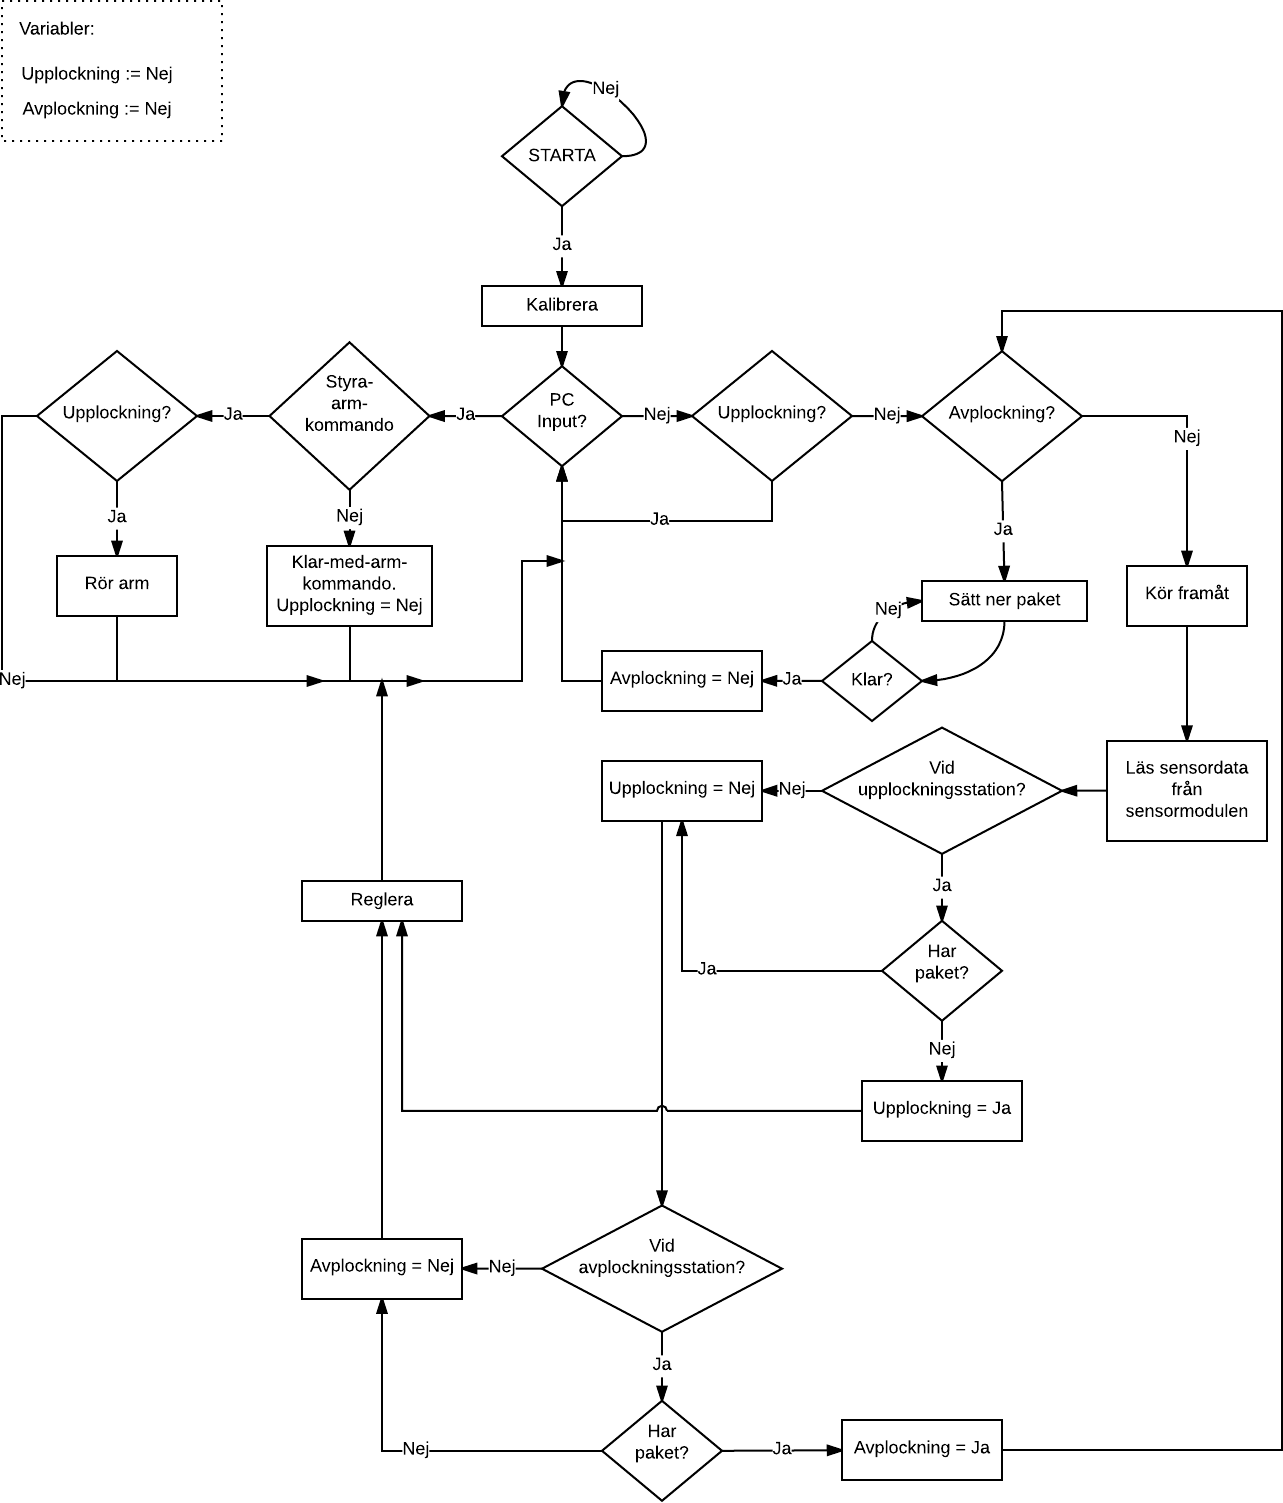
\includegraphics[scale=0.2]{Styrlogik.png}
\caption{Flödesschema för huvudmodulens styralgoritm.} \label{systemskiss:autonomtschema}
\end{figure}

Figur \ref{systemskiss:autonomtschema} är en visualisering av hur det autonoma läget kommer att styras. Med hjälp av två stycken flaggor, Upplockning och Avplockning, kan systemet avgöra om den ska plocka upp eller lämna av ett paket eller bara fortsätta köra framåt längs banan. När Upplockning är satt till "Ja" väntar systemet på att användaren ska styra armen och sedan skicka ett "färdigt-kommando".

\subsubsection{Manuellt läge}
När roboten är satt i manuellt läge väntar huvudmodulen på kommandon från användaren och utför sedan dessa. 

\subsection{Kommunikation}
\subsubsection{Huvudmodul-PC}
\subsubsection{Huvudmodul-Styrenhet}
\subsubsection{Huvudmodul-Sensorenhet}
